\section*{Homework 5}

Do exercise 1-3 from AMPL book

This exercise deals with some issues of sensitivity in the steel models.

\subsection*{A}

\prob

For the linear program of Figures 1-5a and 1-5b, display \texttt{Time} and \texttt{Make.rc}. What do these values tell you about the solution.

\noindent\textbf{Relevant Files:}

\noindent\textbf{steel3.mod}

\begin{lstlisting}
set PROD;  # products

param rate {PROD} > 0;     # produced tons per hour
param avail >= 0;          # hours available in week
param profit {PROD};       # profit per ton

param commit {PROD} >= 0;  # lower limit on tons sold in week
param market {PROD} >= 0;  # upper limit on tons sold in week

var Make {p in PROD} >= commit[p], <= market[p]; # tons produced

maximize Total_Profit: sum {p in PROD} profit[p] * Make[p];

               # Objective: total profits from all products

subject to Time: sum {p in PROD} (1/rate[p]) * Make[p] <= avail;

               # Constraint: total of hours used by all
               # products may not exceed hours available

\end{lstlisting}

\noindent\textbf{steel3.dat}

\begin{lstlisting}
data;

set PROD := bands coils plate;

param:    rate  profit  commit  market :=
  bands    200    25     1000    6000
  coils    140    30      500    4000
  plate    160    29      750    3500 ;

param avail := 40;
\end{lstlisting}

\sol

\textbf{NOTE:} My basic python script for this part is provided in the HW5 appendix at the end of this section.


Running the code, \texttt{ampl.eval("Display Time, Make.rc")}, gives us the output below:

\begin{align*}
	\text{time}_{dv} &= 4640 \\
	\text{bands}_{rc} &= 1.80 \\
	\text{coils}_{rc} &= -3.14 \\
	\text{plates}_{rc} &\approx 0
\end{align*}

The interpretation of these values is as follows. 

First, time. If we were to add an extra unit of time (an hour) to availability we would see additional profit. To be precise we would see an increase of 4640 units of profit (dollar) per additional hour of availability. 

For bands, we see the same kind of thing. Every unit (ton) increase in the upper bound of bands made would see an increase of 1.80 dollars of profit. 

Coils has a negative coefficient. What this means is that every ton decrease in the lower bound of coils made would see an increase in profit by 3.14 dollars. This makes sense, we're maxing out the number of bands we can make and only producing the absolute minimum number of coils. 

Plates have a coefficient of 0, meaning that increasing or decreasing the bounds on its production would have no impact on profit. This also makes sense intuitively as production of plates falls within the provided bounds already. 

It is important to note that for these dual values and reduced costs, this relationship may not hold forever. These values are subject to change as constraints are modified.

\subsection*{B}

\noindent\textbf{Solution:}

The figures mentioned in the problem statement refer to the steel4 data and model files. Those have been shown earlier in the homework so I will not be showing them again. 

\begin{table}[h!]
\centering
\begin{tabular}{lcc}
\hline
 & \textbf{Steel3} & \textbf{Steel4} \\
\hline
Bands  & $6000$       & $\approx 3357.14$ \\
Coils  & $500$        & $500$ \\
Plates & $\approx 1028.57$ & $\approx 3142.86$ \\
Total Profit & $\approx 194828.57$ & $\approx 190071.43$ \\
\hline
\end{tabular}
\caption{Comparison of solution values and total profit for Steel3 and Steel4 models.}
\end{table}

The table for this part show a massive increase in the number of plates produced and a massive decrease in the number of bands. Why is this? 

To explain what's going on here we need to understand the new rate constraint. \texttt{reheat} has the same rate across all 3 products. Previously bands had the highest rate of production which made up for it having the lowest profit coefficient of 2.5. \texttt{reheat}, as mentioned, levels the playing field a bit. Since, for that stage at least, all 3 products have the same rate, the profit coefficient matters a lot more. 

What this means is that plates, with their very high profit coefficient of 2.9, outclass bands for this stage. Bands still come out on top for the rolling stage, which is why we still make so many bands, but this change is why we produce so much less of them. Coils still go completely ignored in this model, we still only produce the bare minimum required. 

\subsection*{C}

\noindent\textbf{Solution}

\textbf{NOTE:} For problems C and D the python script used is provided in the Homework 5 Appendix shown below this problem.

Using \texttt{amplpy} and saving the profit and reheat hours from each run gives us the following table:

\begin{table}[!ht]
    \centering
    \begin{tabular}{lcc}
    \hline
        reheat\_hours & profit & time\_dual\_value \\ \hline
        35 & 190071.43 & 1800.0 \\
        36 & 191871.43 & 1800.0 \\
        37 & 193671.43 & 1800.0 \\
        38 & 194828.57 & 0.0 \\
        39 & 194828.57 & 0.0 \\
        40 & 194828.57 & 0.0 \\
    \hline
    \end{tabular}
\end{table}


This table verifies what the problem statement wanted us to check. We have a constant dual value for reheating up until we hit 38 reheat hours. From there, it has no influence on our profit whatsoever. This is likely due to the constraint on the rolling stage holding back any additional gains from a more generous reheating availability. These just become excess hours that go unused.  

Next we check some other arbitrary values. We start with the provided $37 \frac{9}{14}$. To test this we also solve for $36 \frac{9}{14}$ so compare the dual values. We also test just beyond this value and do the exact same process for $37 \frac{10}{14}$. 

This gives us the following results:

\begin{table}[!ht]
    \centering
    \begin{tabular}{lcc}
    \hline
        reheat\_hours & profit & time\_dual\_value \\ \hline
	$36 \frac{9}{14}$ & 193028.57 & 1800 \\\\ 
	$37 \frac{9}{14}$ & 194828.57 & 0 \\\\
    $36 \frac{10}{14}$ & 193157.14 & 1800 \\\\
	$37 \frac{10}{14}$ & 194828.57 & 0 \\
    \end{tabular}
\end{table}

These tables verify the problem statement. Results below that $37 \frac{9}{14}$ still show that 1800 profit increase. Right as soon as we surpass it even by a tiny amount, the dual value shows us that we would see no additional benefit. 

One interesting observation is that $37 \frac{10}{14}$ doesn't actually see an 1800 profit increase despite the dual value of $36 \frac{10}{14}$. I wonder why that is. It must be that the slope at that point is still 1800, but the tiny part of $37 \frac{10}{14}$ that exceeds our threshold means we don't quite capture 1800 in profit for a one unit increase. Essentially that the slope will flatten out before we see all 1800 dollars of profit realized. This means the dual value doesn't quite tell the whole picture. 

\begin{figure}[htbp]
    \centering
    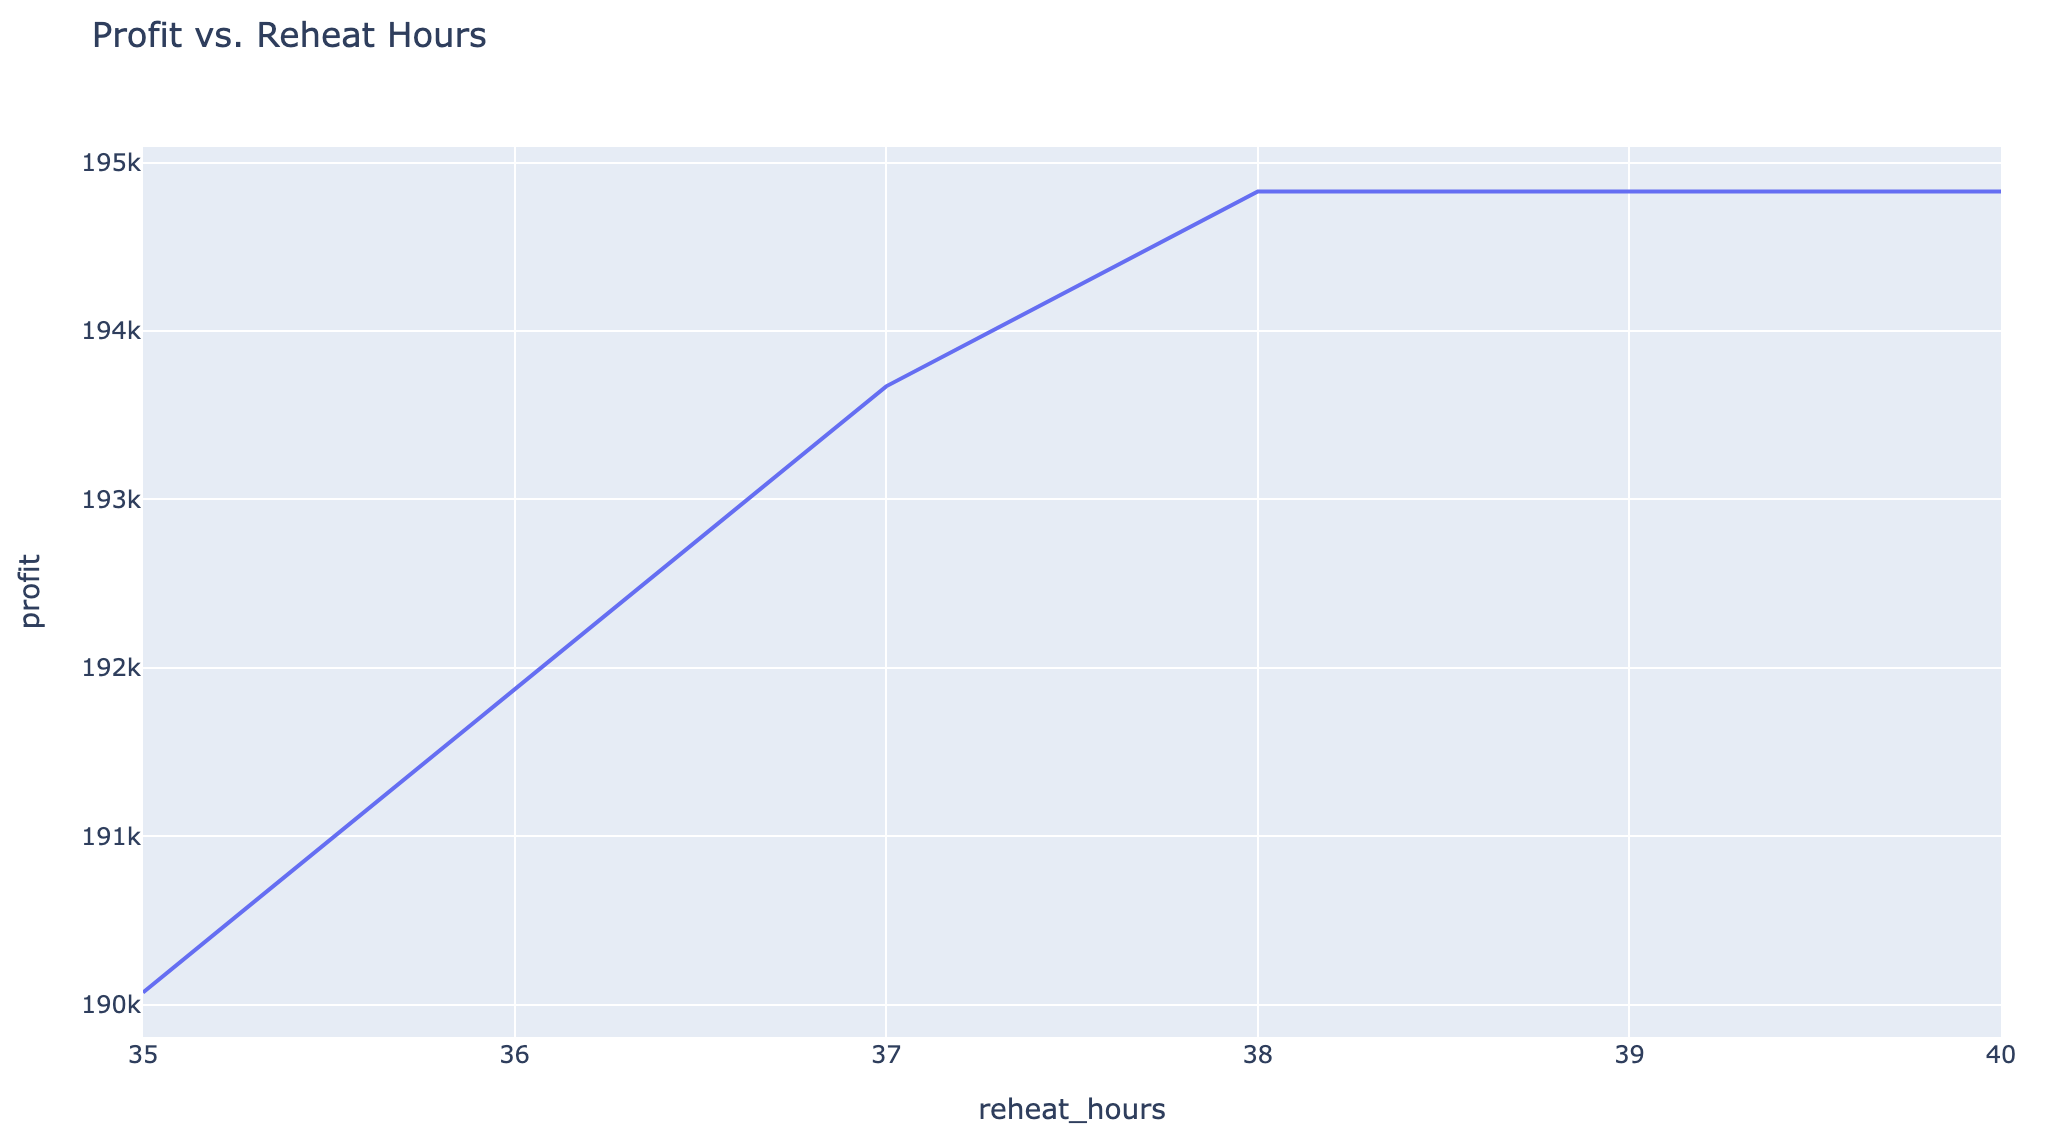
\includegraphics[width=0.8\textwidth]{../images/profit-vs-reheat-1.png}
    \caption{Plot created using the integer range of 35 through 40.}
    \label{fig:your_label}
\end{figure}

The plot here also provides further evidence of this thought. Though it is limited, only showing integer tests from 35-40, we still see that profit starts leveling off more going from 37 to 38. And then, of course, we see no additional gains to profit extending beyond 38 hours. 

\pagebreak

\subsection*{D}

We extend the plot down to 25 reheating hours here.

\begin{figure}[htbp]
    \centering
    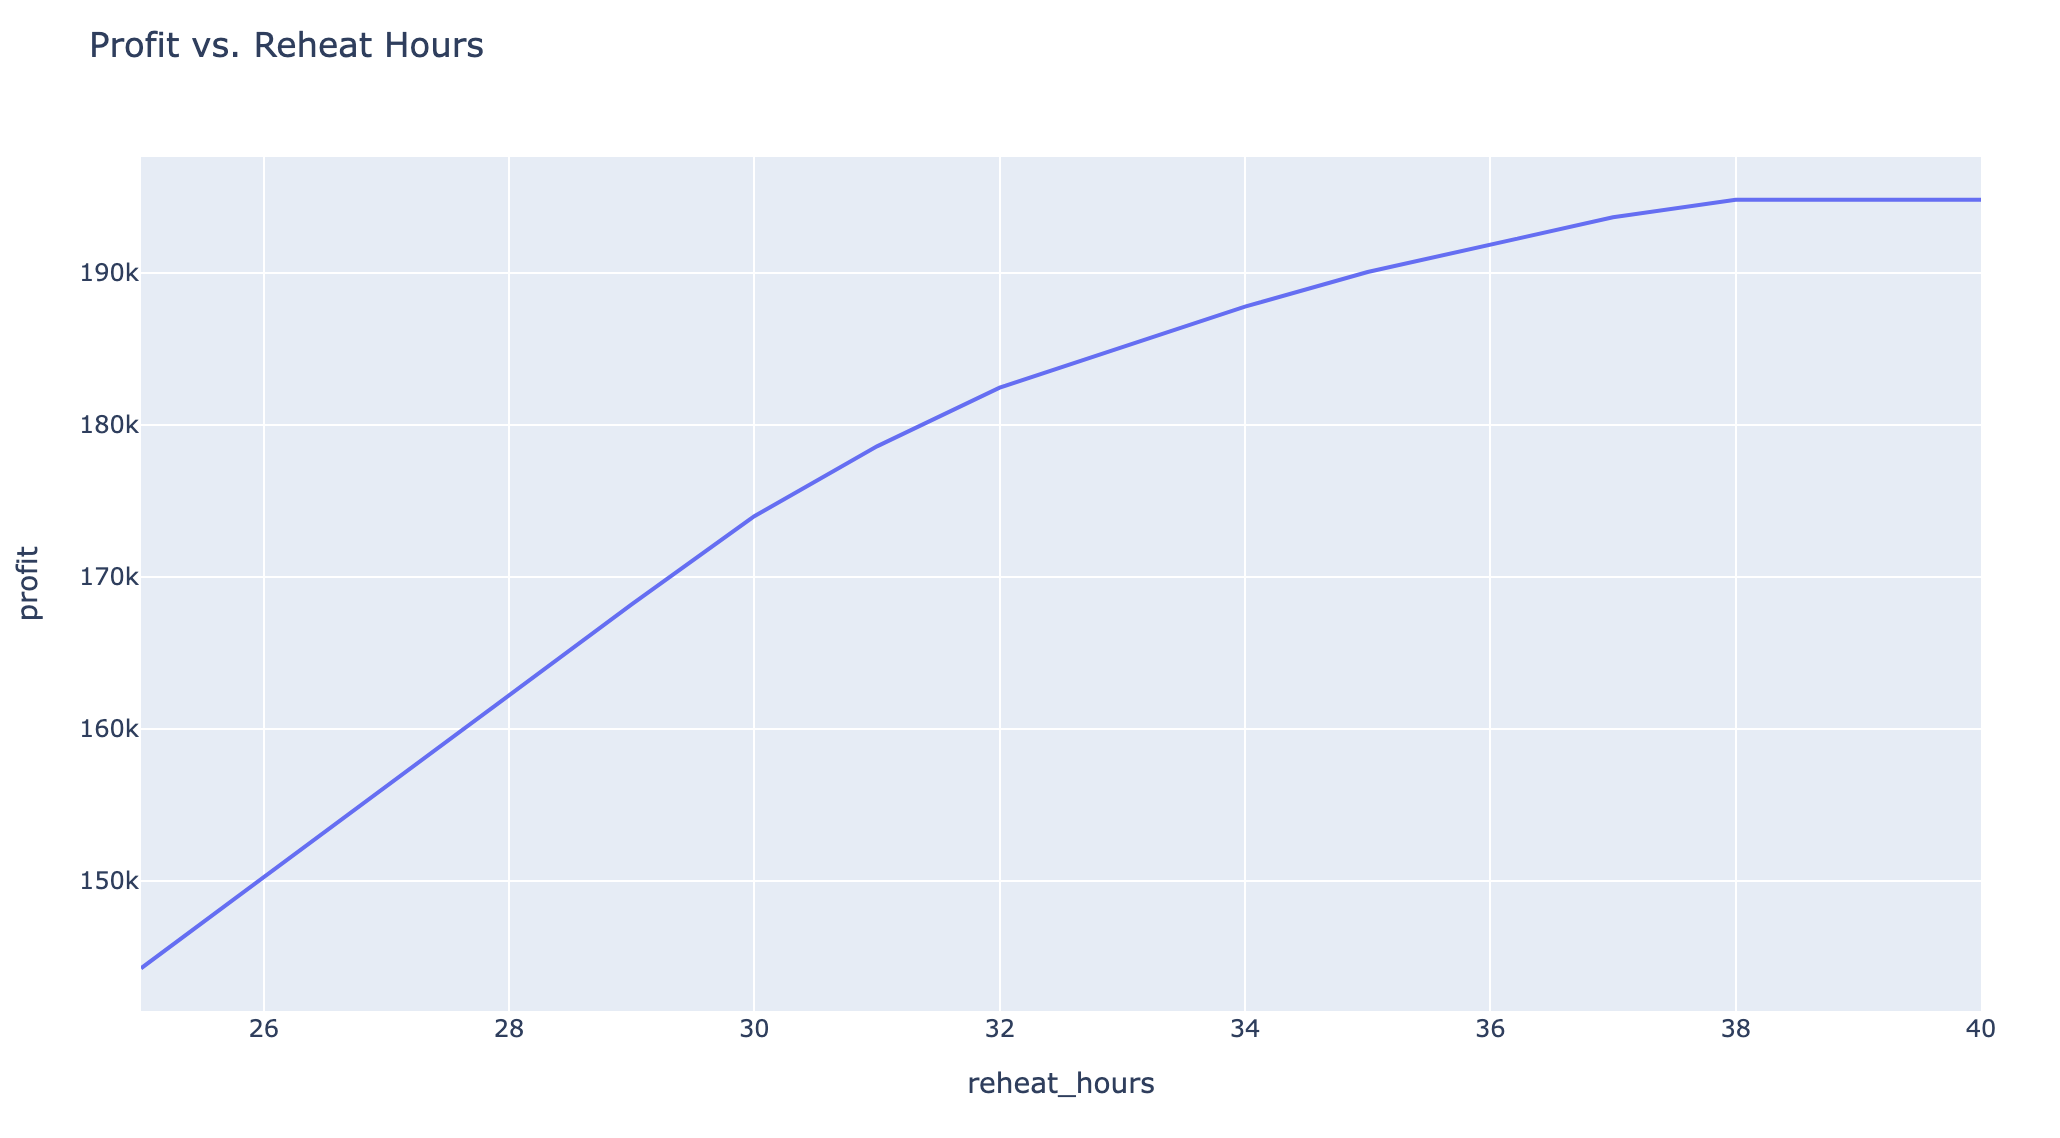
\includegraphics[width=0.8\textwidth]{../images/profit-vs-reheat-2.png}
    \caption{Plot created using the integer range of 25 through 40.}
\end{figure}

Interestingly enough we see the slope had changed well before we hit 35 hours. We see the first changes in the slope of this plot once we hit 30 available hours of reheat time. This isn't surprising. As an untested hunch, this is possibly due to increased access to unused \texttt{rolling} stage availability. With too little \texttt{reheat} availability, we can't properly utilize all of the availability of the other stage. So we see more steep growth early on.

We also extend our table to show all of the profit changes as we move from 10 to 25 available reheating hours.

\begin{table}[!ht]
    \centering
    \begin{tabular}{lcc}
    \hline
        reheat\_hours & profit & time\_dual\_value \\ \hline
        10 & 0.0 & 0.0 \\
        11 & 0.0 & 0.0 \\
        12 & 66250.0 & 6000.0 \\
        13 & 72250.0 & 6000.0 \\
        14 & 78250.0 & 6000.0 \\
        15 & 84250.0 & 6000.0 \\
        16 & 90250.0 & 6000.0 \\
        17 & 96250.0 & 6000.0 \\
        18 & 102250.0 & 6000.0 \\
        19 & 108250.0 & 6000.0 \\
        20 & 114250.0 & 6000.0 \\
        21 & 120250.0 & 6000.0 \\
        22 & 126250.0 & 6000.0 \\
        23 & 132250.0 & 6000.0 \\
        24 & 138250.0 & 6000.0 \\
        25 & 144250.0 & 6000.0 \\
    \hline
    \end{tabular}
\end{table}


Here we have verified that from 12 available reheat hours to 25 hours we see a constant slope of 6000 dollars of profit per hour increase in availability. We also see 0s for 10 and 11 hours of availability. Why is that?

It's because of our minimum production constraints. In the steel4 data file, we have a commit parameter that controls our production lower bounds. We need a minimum of 1000 tons of bands, 500 tons of coils and 750 tons of plates.

Our time constraint is as follows:

\begin{lstlisting}
subject to Time {s in STAGE}:
   sum {p in PROD} (1/rate[p,s]) * Make[p] <= avail[s];
\end{lstlisting}

Running through the math for all products in the reheating stage:

\[
	\frac{1}{200} \cdot (1000 + 500 + 750) = 11.25 > 11
\]

Our minimum production requirements require more than 11 hours of reheating time, so anything below $11.25$ results in no feasible solution being possible. 

\pagebreak
\subsection*{Homework 5 Appendix}

In this section I include python scripts that would be too distracting to include in the homework writeup itself.

Below is the script used for 1-3 part A.

\begin{minted}[fontsize=\small,breaklines,linenos]{python}
from amplpy import AMPL
from loguru import logger

def main():
    logger.info("Initializing solver")
    ampl = AMPL()
    ampl.setOption("solver", "highs")

    file_name = "steel3"
    logger.info("Reading data")
    ampl.read(f"../models/{file_name}.mod")
    ampl.read_data(f"../data/{file_name}.dat")

    logger.info("Running solution")
    ampl.solve()
    ampl.eval("display Time, Make.val, Make.rc;")

if __name__ == "__main__":
    main()
\end{minted}

Below is the script used for 1-3 parts C and D.

\begin{minted}[fontsize=\small,breaklines,linenos]{python}
from amplpy import AMPL
from loguru import logger
import polars as pl
import plotly.express as px

def main(reheat_hours_list):
    file_name = "steel4"
    profit_list = []
    duals = []

    # Goal here is to populate a dataframe we can examine through all of the necessary runs
    # We initiate AMLP() in this loop so thats its fully reset between runs.
    # Not doing this can result in weird results for edge case scenarios.
    for reheat_hours in reheat_hours_list:
        logger.info("Initializing solver")
        ampl = AMPL()
        ampl.setOption("solver", "highs")
        logger.info("Reading data")
        ampl.read(f"../models/{file_name}.mod")
        ampl.read_data(f"../data/{file_name}.dat")
        logger.info(f"Solving with reheat availability = {reheat_hours}")
        ampl.getParameter("avail")["reheat"] = reheat_hours
        ampl.solve()

        profit = ampl.getObjective("Total_Profit").value()
        profit_list.append(round(profit, 2))

        # Dual value (shadow price) for the reheat stage
        dual_value = ampl.getConstraint("Time")["reheat"].dual()
        duals.append(round(dual_value, 2))

    df = pl.DataFrame({
        "reheat_hours": reheat_hours_list,
        "profit": profit_list,
        "time_dual_value": duals
    }, strict=False)


    return df


if __name__ == "__main__":
    reheat_hours_list = list(range(10, 41))
    # test_value_1 = 37 + (9/14)
    # test_value_2 = 37 + (10/14)
    # reheat_hours_list = [test_value_1 - 1, test_value_1, test_value_2 - 1, test_value_2]
    # reheat_hours_list = [test_value_1, test_value_2]

    df = main(reheat_hours_list)
    with pl.Config(tbl_rows=40):
        print(df)
    df.write_csv("../data/reheat-profit-table.csv")

    # fig = px.line(df, x="reheat_hours", y="profit, title='Profit vs. Reheat Hours')
    # fig.show()
\end{minted}

